\chapter{Dynamo}

\paragraph{How would you describe Dynamo} Dynamo is used to manage the state of
services that have very high reliability requirements and need tight control
over the tradeoffs between availability, consistency, cost-effectiveness and
performance; services that only need primary-key access to a data store.

\paragraph{System design} Only used internally by Amazon originally, all nodes
are assumed to be trusted. Target of 300ms (for 99.9\% of incoming reqs) at peak
rate of 500 requests/s.
\begin{itemize}
  \item \textbf{Query Model}: Simple read and write operations to a (usually
    small) data item uniquely identified by a key.
  \item \textbf{ACID}: Trade consistency. All updates eventually reach all
    replicas.
  \item \textbf{Efficiency}: Optimise for 99.9th percentile of \textbf{latency}
    over performance, cost efficiency, availability, and durability guarantees.
  \item \textbf{Always writable}: Conflict resolution happens on reads. Can be
    handled by dynamo (latest write) or application (e.g merge shopping carts).
  \item \textbf{Scalability}: Should be able to add one node at a time with
    minimal impact. Load should be balanced across \textbf{heterogeneous} nodes.
  \item \textbf{Decentralisation}: Favour peer to peer techniques and assume all
    nodes are \textbf{symmetric} (can take any set of responsibilities). This is
    to make operation as easy as possible.
  \item \textbf{Zero-hope DHT}: Each node maintains routing information locally
    (optimised for latency).
\end{itemize}

\paragraph{Partitioning and replication} \textbf{Key}: MD5 hash to determine
node serving it.
\begin{itemize}
  \item \textbf{Partitioning}: Consistent hashing (in a ring). Nodes responsible
    for range of keys before itself, until its predecessor(s) node on the ring.
  \item \textbf{Virtual nodes} Makes partitioning optimisable. Give physical
    nodes ``tokens'' to VNs.
    \begin{itemize}
    \item[$+$] Dynamic range: can adapt based on physical node capacity
    \item[$+$] Makes it easy to spread load on failure/node addition.
    \end{itemize}
  \item \textbf{Replication}: Replication on N hosts defined per intance. Each
    key $k$ assigned to coordinator VN and replicated to the next N-1
    \textbf{PNs} on the ring (and spread across DCs). Those nodes are first in
    $k$'s \emph{preference list}.
\end{itemize}

\paragraph{Versioning} Vector clock for automatic resolution of causally ordered
updates. Vector clocks are garbage collected after reaching a certain size which
could technically cause issues. If automatic reconciliation cannot be applied
then fall back to returning all results and apply decided scheme.

\paragraph{Execution} One coordinator talks to client and handles internal
communication.
\begin{itemize}
\item \textbf{Client}: Request is routed through a load balancer, or client is
  aware of key distribution.
  \item \textbf{Quorum}: For consistency, require R nodes to participate in read
    req and W nodes in write req. Latency of req is one of slowest node. Setting
    R=1 makes for very fast reads.
  \item \textbf{Sloppy Quorum}: For get, assume N = W. If any node in pref list
    fails then we are unavailable. Get another node to write locally, and then
    when node goes back up/new node added pass the local write to it. If this
    node fails as well, then the anti-entropy system using \textbf{Merkel trees}
    will ensure this update still reaches the recovered node.
\end{itemize}

\paragraph{Physical node} By symmetry, each node does a lot
\begin{itemize}
  \item \textbf{Membership}: Gossip based protocol for membership (eventually
    consistent). Local idea of failure (if I can't talk to X then I will
    consider it failed temporarily - good for latency) and gossip about it.
    Formal node addition and removal methods ensure global view is correct
    (e.g. count to infinity problem).
  \item \textbf{Storage}: Different local storage options, possible persistent
    in-memory store.
  \item \textbf{Request coordination}: State machine contains all logic for
    identifying nodes responsible for key, sending requests, waiting for
    responses, retries, processing retries, packaging response. One SM per req.
\end{itemize}

\paragraph{Performance} Can choose R, W depending on wanted performance. Dynamo
also lets you write only to memory buffer (N-W node will still write to disk for
durability, but no need to wait for them).

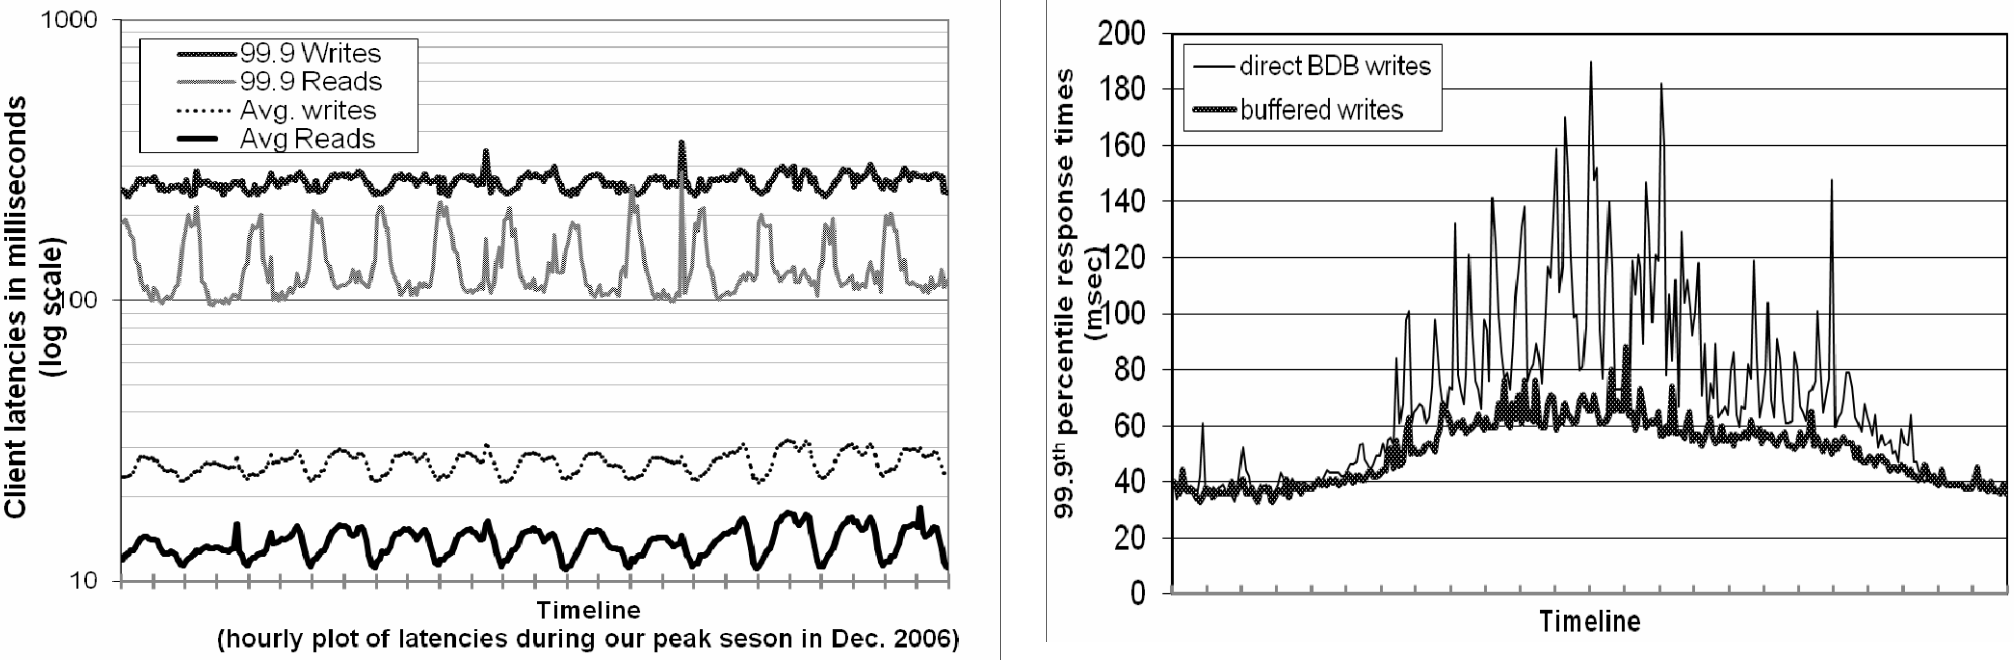
\includegraphics[width=0.98\linewidth]{img/dyn-perf.png}

\paragraph{Uniform load distribution}. Assumption: Even if there is a skew in
the access distribution, there are enough keys in the popular end of the
distribution so that the load of handling popular keys can be spread across the
nodes uniformly through partitioning. Distributing keys based on load is hard
because we need the zero-hop property to hold.
\begin{itemize}
  \item \textbf{Partition by Token value}: bad because data partitioning and
    data placement are intertwined. Leads to high data replication cost when
    adding new machines
  \item \textbf{``Random'' Equal sized partitions}: Could spread loaded
    partitions. But high overhead because of repartition needs to be exchanged
    all the time.
  \item \textbf{Equal sized partitions}: $\frac{\textrm{\#partitions}}{\textrm{\#nodes}}$ per
      node. When adding or removing a node, each node need to steal or give off
      a bit of its range (but that requires coordination).
\end{itemize}

\newpage
\paragraph{Questions}: How does Dynamo handles partitioning, replication,
versioning, membership, failure handling and scaling? And can you explain the
table below?

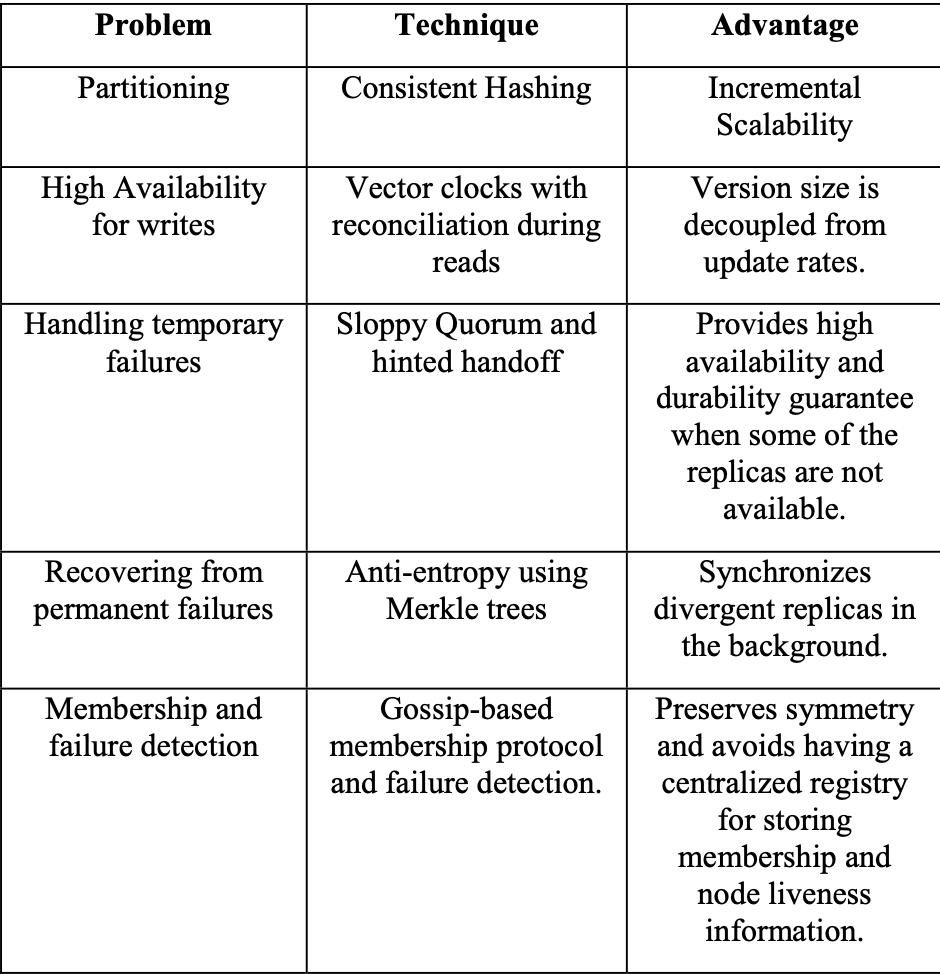
\includegraphics[width=0.45\linewidth]{img/dyn-tech.png}
